\textbf{See the instruction for questions \inteval{\value{question}+1} to \inteval{\value{question}+3}.}

\begin{figure}[H]
\centering
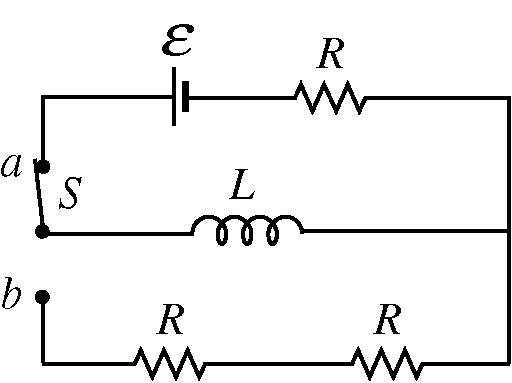
\includegraphics[scale=0.25]{images/img-007-022.png}
\end{figure}

In the circuit above, all of the resistors have the same resistance $R$. Switch $S$ has been in position $a$ for a very long time.

% Multiple Choice Question 11
\begin{questions}\setcounter{question}{10}\question
What is the energy stored by the inductor?

\begin{oneparchoices}
\choice Zero
\choice $\dfrac{\mathcal{E}^{2}}{R}$
\choice $\dfrac{1}{2} L \mathcal{E}^{2}$
\choice $\dfrac{1}{2} L \dfrac{\mathcal{E}}{R}$
\choice $\dfrac{1}{2} L \dfrac{\mathcal{E}^{2}}{R^{2}}$
\end{oneparchoices}\end{questions}

% Multiple Choice Question 12
\begin{questions}\setcounter{question}{11}\question
The switch is now moved instantaneously to position $b$. The voltage across the inductor immediately after the move is

\begin{choices}
\choice zero
\choice greater than zero but less than $\mathcal{E}$\choice $\mathcal{E}$
\choice greater than $\mathcal{E}$ but not infinite
\choice infinite
\end{choices}\end{questions}

% Multiple Choice Question 13
\begin{questions}\setcounter{question}{12}\question
The time constant when the switch is in position $a$ is $\tau_{0}$. How does the time constant when the switch is in position $b$ compare to $\tau_{0}$ ?

\begin{choices}
\choice It is zero.
\choice It is less than $\tau_{0}$ but greater than zero.
\choice It is equal to $\tau_{0}$.
\choice It is greater than $\tau_{0}$ but not infinite.
\choice It is infinite.
\end{choices}\end{questions}

